
%\documentclass[10pt,twoside,twocolumn]{article}
\documentclass[10pt,twoside]{article}
\usepackage[bf,small,nooneline]{caption}
\usepackage[letterpaper,hmargin=1in,vmargin=1in]{geometry}
\usepackage{paralist} % comapctitem, compactdesc, compactenum
\usepackage{titlesec}
\usepackage{titletoc}
\usepackage{times}
\usepackage{hyperref}
%\usepackage{glossaries}
%\usepackage[xindy]{glossaries}
%\usepackage[toc]{glossaries}
\usepackage{graphicx}
\graphicspath{{./graphics/}}
\usepackage{xspace}
\usepackage{verbatim}
\hyphenation{Sub-Bytes Shift-Rows Mix-Col-umns Add-Round-Key}

\newcommand{\bulk}{\emph{bulk\_extractor}\xspace}
\newcommand{\bev}{\emph{BEViewer}\xspace}
%\newcommand{\button}[1]{(\raisebox{-1.20mm}{\includegraphics[scale=0.90]{./graphics/#1}})}

\begin{document}

%\titlespacing{\section}{0pt}{0pt}{0pt}
%\titlespacing{\subsection}{0pt}{0pt}{0pt}
%\titlespacing{\subsubsection}{0pt}{0pt}{0pt}
%\date{}

\title{Bulk Extractor Viewer (\bev) Summary}
%\author{Bruce Allen \footnote{\href{mailto:bdallen@nps.edu}{bdallen@nps.edu}}}
\maketitle

%\begin{abstract}
%  The Bulk Extractor Viewer (\bev)
%  is a User Interface for browsing Feature data extracted
%  using the \bulk extraction tool.
%  In addition to browsing Features,
%  \bev provides facilities for viewing multiple Images,
%  managing Feature sets as work settings,
%  and exporting Bookmarked Features.
%\end{abstract}

%%\newpage
%\cleardoublepage
%\setcounter{tocdepth}{2}
%\tableofcontents
%%\newpage
%\cleardoublepage

\section{The Main \bev Screen}
A sample \bev screenshot showing a navigated Feature is shown in Figure~\ref{bev-example}.
\begin{figure}[h]
\center
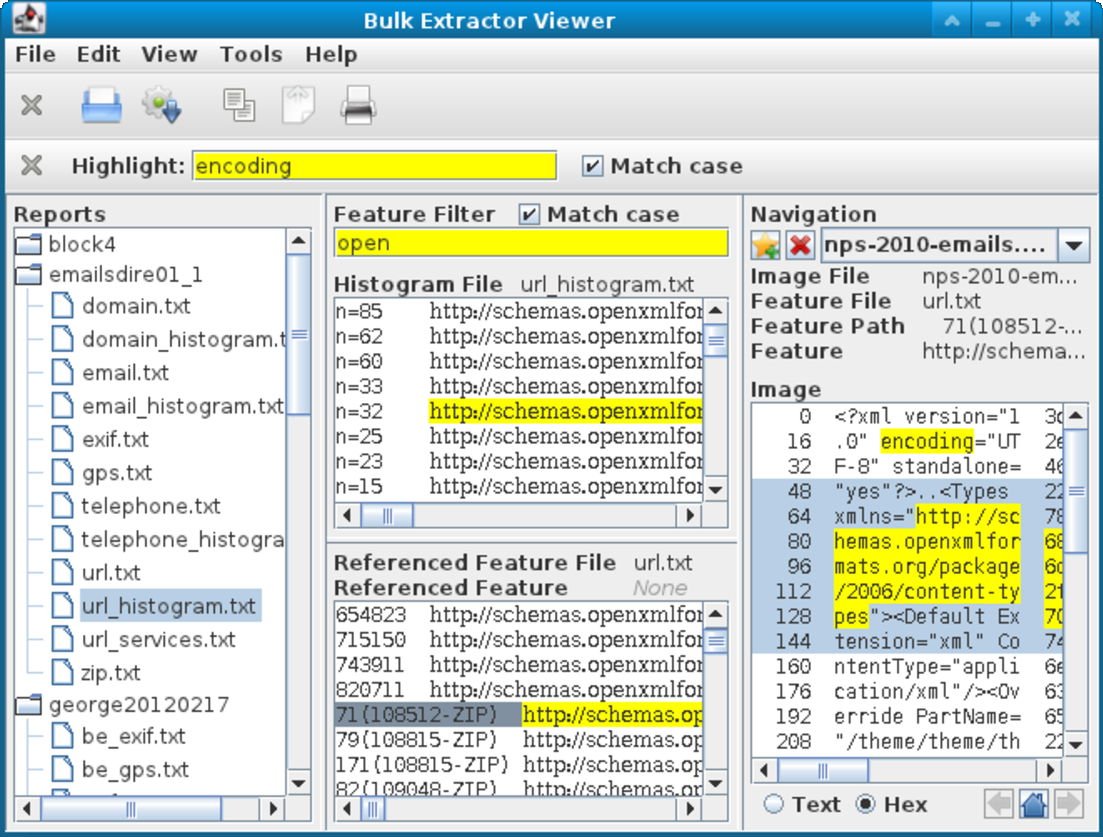
\includegraphics[scale=0.4]{images/BEViewer_example}
\caption{Sample \bev screenshot.\label{bev-example}}
\end{figure}

A blank \bev screenshot with areas labeled is shown in Figure~\ref{bev-blank-annotated}.
\begin{figure}[h]
\center
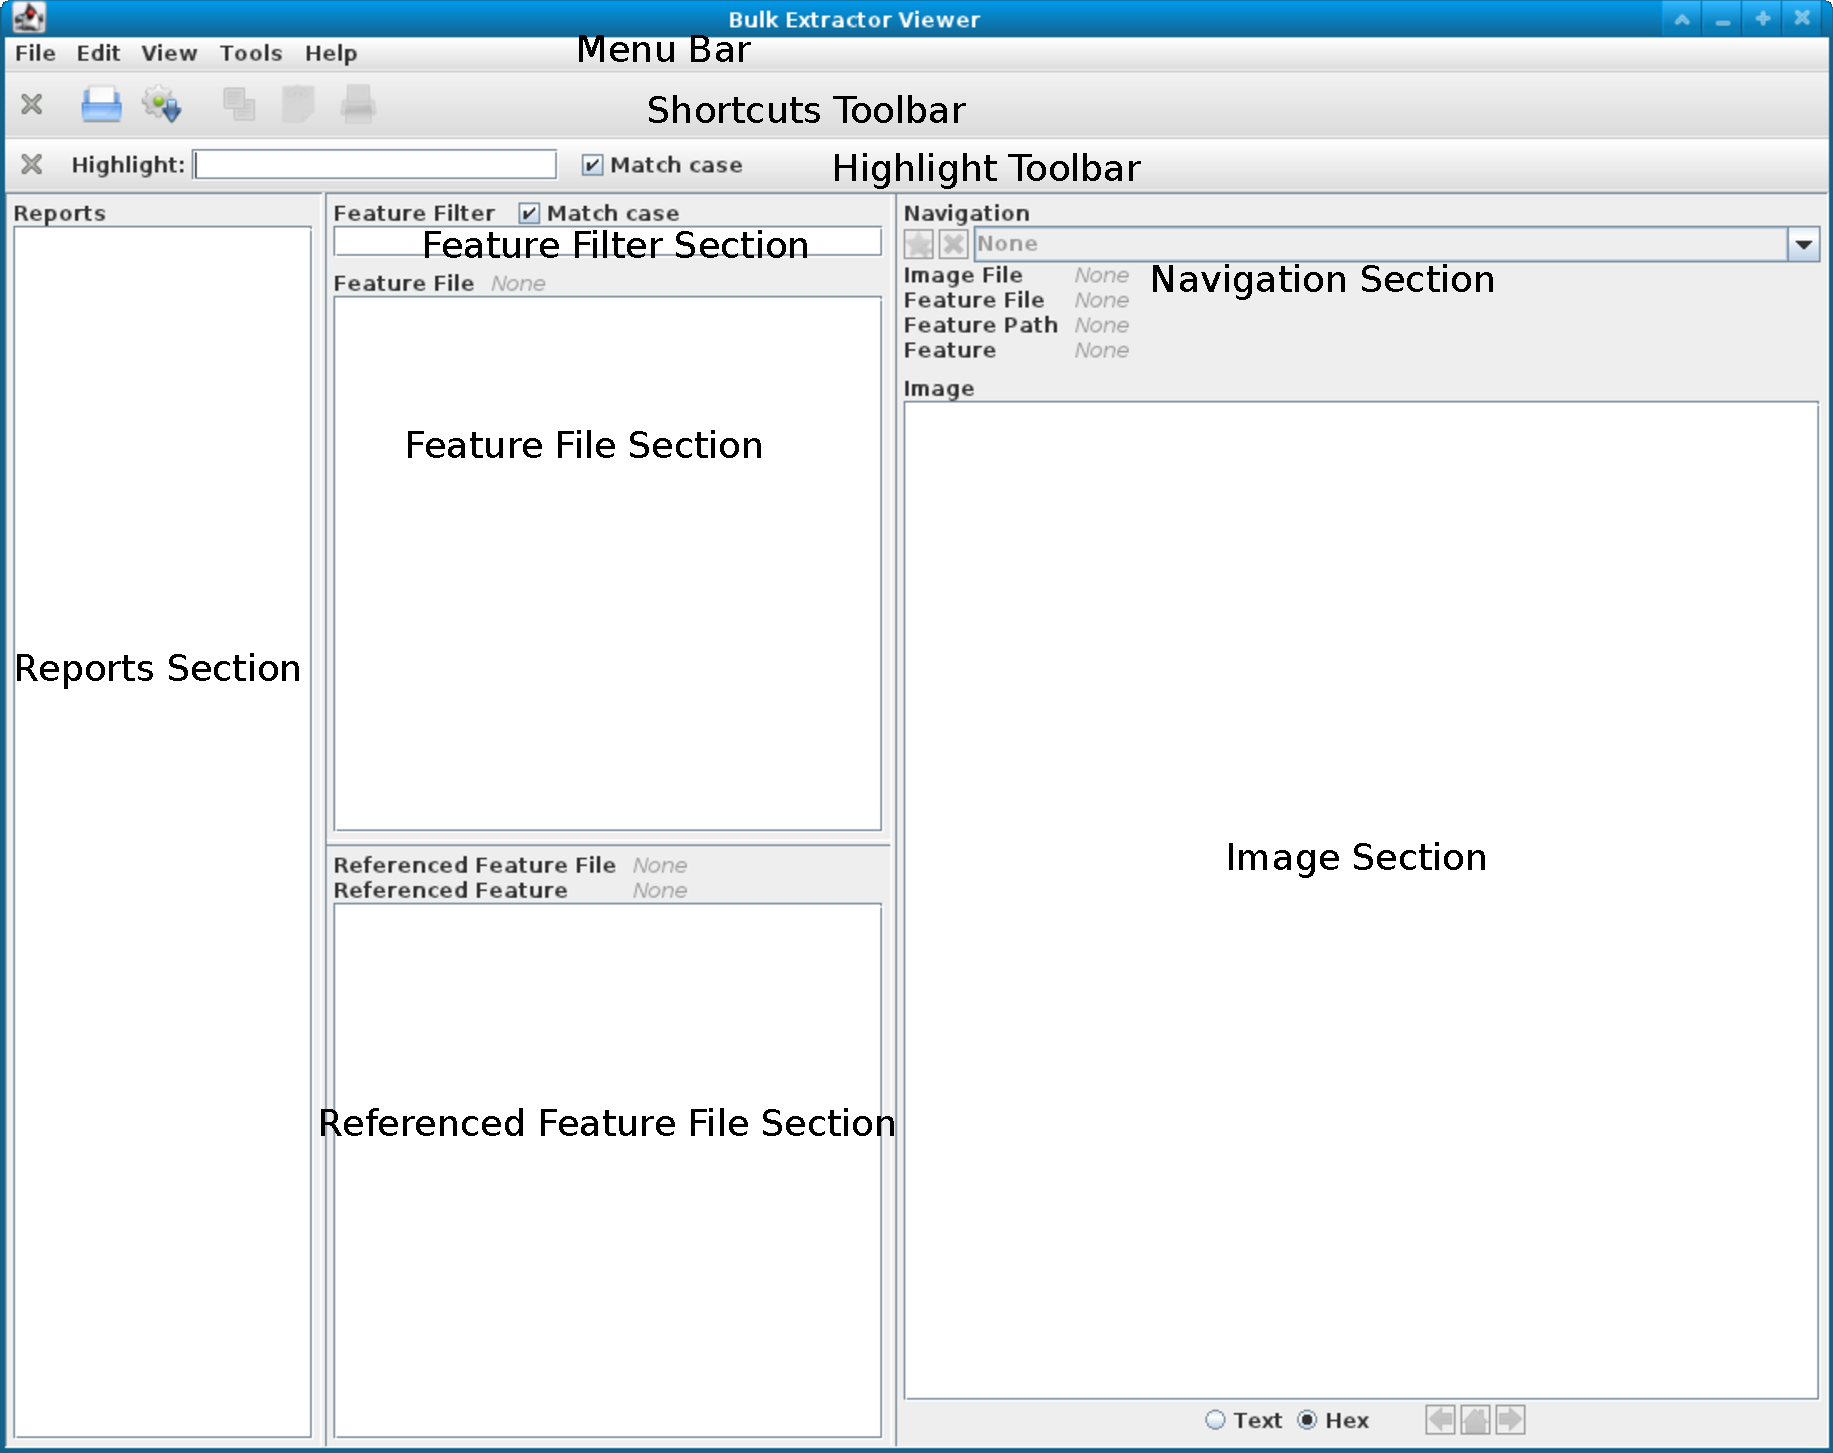
\includegraphics[scale=0.25]{images/BEViewer_blank_annotated}
\caption{Blank \bev screenshot with sections annotated.\label{bev-blank-annotated}}
\end{figure}

The main \bev screen is described in sections:
% Menu Bar
\subsection{Menu Bar}
Menus provide controls for \bev such as opening Reports, managing Bookmarks,
copying ranges, configuring views, and running \bulk:
\begin{compactitem}
\item Use \texttt{File} to manage Reports, Bookmarks, and Work Settings, and to print or quit.
\item Use \texttt{Edit} to Copy and to clear the Navigation history.
\item Use \texttt{View} to set view parameters and to view properties.
\item Use \texttt{Tools} to run \bulk.
\item Use \texttt{Help} for Help, version information, logs, and diagnostics.
\end{compactitem}
% Shortcuts toolbar
\subsection{Shortcuts Toolbar}
The Shortcuts toolbar provides the following shortcuts:
\begin{compactitem}
\item Open Report for browsing its Features.
\item Run \bulk to scan an Image and create Feature files containing Features from that Image.
\item Copy a range of Features or a range of Image lines
that have been selected by dragging the mouse over them.
\item Export bookmarks to a file.
\item Print the selected Feature range or Image range.
\end{compactitem}
% Highlight toolbar
\subsection{Highlight Toolbar}
The Highlight toolbar allows typed text to be highlighted in the Feature and Image areas:
\begin{compactitem}
\item Highlights show up in the Feature File listings and in the Image listing.
\item Multple highlights may be issued by separating them with the \textbar \xspace character.
\item Unusual characters may be highlighted by entering their escaped octal sequences,
for example \texttt{\textbackslash 000}.
\item Click the Match case checkbox to match capitalization.
\end{compactitem}
% Reports section
\subsection{Reports Section}
The Reports section is used to select Feature files from an opened Report.
\begin{compactitem}
\item Hover over a Report folder to see the Report directory
and the Image file associated with the Report.
\item Hover over a Feature file or Histogram file to see the full path to it.
\begin{compactitem}
\item Feature files contain feature entries organized by filename.
\item Feature filenames ending in \texttt{\_histogram.txt} contain histogram information.
\item Empty files and Stoplist files may be suppressed or shown.
\end{compactitem}
\item Click on a Report folder to see the Feature files within it.
\item Click on a Feature file to view the Features within it.
\item Click on a Histogram file to view the histogram entries in the Histogram listing
and view the associated Feature file in the Referenced Feature file listing.
\item When a folder or file is selected,
you may use menu action \texttt{File \textbar \xspace Close Report} to close it.
\end{compactitem}
% Feature Filter
\subsection{Feature Filter Section}
The Feature Filter filters what Features are shown in the Feature file or Histogram file area.
\begin{compactitem}
\item Type text to apply a filter.
\item Click the Match case checkbox to match capitalization.
\end{compactitem}
% Feature File
\subsection{Feature File Section}
If a Feature file is selected in the Reports section then its features are displayed:
\begin{compactitem}
\item Click on a Feature to navigate to it.
\item Drag on a range to select the range.
\item Press the Escape key to deselect the range.
\end{compactitem}
If a Histogram file is selected in the Reports section then the histogram entries
associated with the Histogram file are displayed:
\begin{compactitem}
\item Click on a Histogram entry to display the Features associated with this Histogram entry
in the Referenced Feature File section.
\item Press the Escape key to deselect the Histogram entry.
Note that the Referenced Feature File section goes back to displaying all features
instead of displaying the associated ones.
\item Drag on a range to select the range.
\item Press the Escape key to deselect the range.
\end{compactitem}
Additionally:
\begin{compactitem}
\item Type filter text to filter the set of features that are displayed.
\item Type highlight text to highlight specific features.
\end{compactitem}
% Referenced Feature File
\subsection{Referenced Feature File Section}
The Referenced Feature File section is only used when a Histogram file is selected
in the Reports section.
The Referenced Feature file shown is the Feature file corresponding to the Histogram file selected.
\begin{compactitem}
\item Click on a Feature to navigate to it.
\item Drag on a range to select the range.
\item Press the Escape key to deselect the range.
\end{compactitem}
The set of features displayed in the Referenced Feature File listing
depends on whether a histogram entry is selected in the Histogram area:
\begin{compactitem}
\item If no histogram is selected, all feature entries are shown
in the Referenced Feature File listing.
\item If a histogram entry is selected,
only features matching that of the histogram entry are shown
in the Referenced Feature File listing.
\end{compactitem}

% Navigation
\subsection{Navigation Section}
The Navigation section controls which Feature is currently navigated to.
\begin{compactitem}
\item Click the Bookmark button to bookmark the Feature that is currently navigated to.
\item Click the Delete button to deselect the Feature that is currently navigated to
and to delete it from the Navigation list.
\item Select another feature in the Navigation list to navigate to that feature.
\item The Image File, Feature File, Feature Path, and Feature labels
indicate attributes about the feature that is currently navigated to.
\end{compactitem}
% Image
\subsection{Image Section}
The Image section displays a page of the image
associated with the feature that is currently navigated to.
\begin{compactitem}
\item Drag on a range to select the range.
\item Press the Escape key to deselect the range.
\item Press the Text or Hex button to view the image as text or as hexadecimal bytes.
\item Press the Forward, Reverse, and Home buttons to page forward and back in the image data.
\end{compactitem}
% Sample Screenshot Explained
\subsection{Sample \bev Screenshot Explained}
The sample screenshot shown in Figure~\ref{bev-example} has the following going on:
\subsubsection{Shortcuts Toolbar}
The Shortcuts toolbar indicates the following:
\begin{compactitem}
\item More Reports can be opened for browsing.
\item The \bulk scanner can be run.
\item A range selection has been made in the Image section
that may be copied to the System Clipboard.
\item Features have been bookmarked and these bookmarks can be exported.
\item A range selection has been made in the Image section that may be printed.
\end{compactitem}
\subsubsection{Highlight Toolbar}
Highlighting is in effect because there is text, in this case \texttt{encoding},
in the highlight field.
\begin{compactitem}
\item Highlighting is not shown in either Feature listing
because the word \texttt{encoding} is not present in either of them.
\item Highlighting is shown in the Image view.
\item The highlighting case is set so that capitalization must match.
\end{compactitem}
\subsubsection{Reports Section}
The Reports section indicates the following:
\begin{compactitem}
\item Three reports are visible in the Reports tree, two of which are expanded.
\item Within the \texttt{emailsdire01\_1} Report,
histogram feature file \texttt{url\_histogram.txt} is selected.
\end{compactitem}
\subsubsection{Feature Filter Section}
Feature filtering is in effect because there is text, in this case \texttt{open},
in the filter field.
\begin{compactitem}
\item Feature filtering filters the features shown
in the Feature File listing or the Histogram file listing.
\item Feature filtering does not filter features shown in the Referenced Feature File listing.
\item The filtering case is set so that capitalization must match.
\end{compactitem}
\subsubsection{Feature File Section}
\begin{compactitem}
\item In this example, the Feature File section contains features
from Histogram file \texttt{url\_histogram.txt}
selected from the Reports pane.
\item Only features containing text \texttt{open} are shown
because the Feature File section is being filtered.
\item No histogram entry is selected.
\item One histogram entry is highlighted
because it matches the feature that is selected in the Referenced Feature File area.
\end{compactitem}
\subsubsection{Referenced Feature File Section}
\begin{compactitem}
\item Referenced Feature file \texttt{url.txt} is shown
because Histogram file \texttt{url\_histogram.txt} is selected in the Reports section.
\item The Feature at path \texttt{71(108512-ZIP)} is selected.
As a result:
\begin{compactitem}
\item The feature is selected.
\item The feature's text is highlighted
in the Feature File section, the Referenced Feature File section,
and in the Image section.
\end{compactitem}
\end{compactitem}
\subsubsection{Navigation Section}
The Navigation section shows that a feature has been navigated to.
\begin{compactitem}
\item The Navigation History drop-down box shows the feature that is navigated to.
\item Navigation attributes indicate
the Image file, Feature file, Feature path, and Feature text
associated with the feature that is navigated to.
\end{compactitem}
\subsubsection{Image Section}
\begin{compactitem}
\item The Image section displays the page of image data
corresponding to the selected Feature.
\item A range of rows is selected and it may be copied to the System Clipboard or printed.
\item Text \texttt{encoding} is highlighted as requested in the Highlight Toolbar.
\item Feature text is highlighted because it is selected.
\item A hexadecimal view of the image is displayed because the Hex view is selected
as opposed to the Text view.
\item Forward and back buttons are disabled because they are not useful:
the un-zipped content at this path all fits on one page.
\end{compactitem}

\section{\bev Facilities}
% Generating Reports
\subsection{Generating Reports}
\bulk creates a report of features by running scanners on media images.
A Report consists of:
\begin{compactitem}
\item The directory containing the report.
\item The \texttt{report.xml} text file that \bulk creates when performing the scan.
\item Text files, ending in \texttt{.txt}, containing features found during the \bulk scan:
\begin{compactitem}
\item Feature files.
\item Histogram files generated from feature files,
typically containing \texttt{\_histogram} in their filename.
\item Stoplist files, if a stoplist is used,
which contain features that have been excluded from the feature files.
These end in \texttt{\_stoplist.txt}.
\end{compactitem}
\end{compactitem}
Generate Reports by running the \bulk scanner one of these ways:
\begin{compactitem}
\item Click on the Run \bulk button.
\item Run \bulk outside of \bev at the command prompt.
\item Run \bulk automatically when starting \bev by starting \bev using the \texttt{-r} option.
\end{compactitem}
% Managing Reports
\subsection{Managing Reports}
\bev displays Features in Reports created by running the \bulk scanner.
Reports must be opened so that \bev can view their Features.
\begin{compactitem}
\item Open Reports that have been created by \bulk.
\item Reports are opened automatically when they are created by running \bulk from \bev.
\item Close Reports to remove them from the Reports listing and from any Navigation history.
\end{compactitem}
% Bookmarks
\subsection{Bookmarks}
Features may be bookmarked.
\begin{compactitem}
\item Bookmarks are made by clicking on the Bookmark button.
\item Bookmarked features may be exported to a file.
Bookmark files show properties of bookmarked features along with their corresponding Image data.
\end{compactitem}
% Feature Formats
\subsection{Feature Formats}
Features are extracted from their native encodings in the image.
For example:
\begin{compactitem}
\item Email addresses are often found in binary format or in UTF-16 format.
\item IP addresses are obtained from specific bytes
where surrounding bytes match an identifying pattern.
\end{compactitem}
\bulk scanners find these features, extract them, format them according to their type, then write them to their corresponding Feature file
where they can be viewed directly, imported into Excel, or accessed by Python scripts and by \bulk.

\bulk formats features from Feature files based on their feature type for the following purposes:
\begin{compactitem}
\item \bulk reformats feature contents so that features may be displayed as a summary on one line.
\item \bulk creates a highlight template
so that image bytes that map to features may be highlighted.
\end{compactitem}
% Highlighting
\subsection{Highlighting}
Highlighting in \bev comes from two sources:
\begin{compactitem}
\item Text typed in the Highlighting Toolbar.
\item Feature content associated with the currently selected feature.
\begin{compactitem}
\item For Feature views, feature highlighting consists of the formatted feature text.
\item For the Image view, feature highlighting is based on the highlighting template
corresponding to the feature type.
\end{compactitem}
\end{compactitem}
Highlighting shows up in three places:
\begin{compactitem}
\item The Feature File area.
\item The Referenced Feature File area.
\item The Image area.
\end{compactitem}
To support highlighting of unusual characters and bytes,
highlighting may be entered using escaped octal sequences,
for example \texttt{\textbackslash 000}.
% Work Settings
\subsection{Work Settings}
Work settings contain setting information
about what Reports are currently opened and what Bookmarks are currently selected.
Work settings allow you to add saved information to your work settings
or to move them to another computer.
\begin{compactitem}
\item Export Work Settings to a file.
\item Import Work Settings from a file, augmenting existing work settings.
\item Import Work Settings from a file, replacing existing work settings.
\end{compactitem}
% Clipboard
\subsection{Clipboard}
Copy information to the System Clipboard so that it may be pasted elsewhere.
\begin{compactitem}
\item Copy a Feature, Histogram, or Image range selection.
\item Copy the \bev runtime log so that it can be pasted into a failure report.
\end{compactitem}
% Print output
\subsection{Printing Output}
Print a feature or image range selection:
\begin{compactitem}
\item Select a range and then click on the Print button to print the range.
\item Press the Escape key to deselect the range.
\end{compactitem}
% Usage
\subsection{Command-line Usage}
\bev accepts input parameters when it is started from the command line:
\begin{compactitem}
\item Type \texttt{-s "<scanner arguments>"}, quotes included, to start the \bulk scanner
with scanner arguments that are provided to \bulk.
\item Type \texttt{-clear\_preferences} to reset all user preferences saved previously by \bev.
\end{compactitem}

\end{document}
